\documentclass[10pt,twocolumn]{article}

% use the oxycomps style file
\usepackage{oxycomps}
\usepackage{xcolor}
\addbibresource{ref.bib}


\title{OxyGPT - Creating a large language model for Occidental College}
\author{Zahir Choudhry}
\affiliation{Occidental College}
\email{zchoudhry@oxy.edu}
\date{May 2024}

\begin{document}

\maketitle

\section{Abstract}
Large language models are becoming the mainstream way to consume information. This paper proposes the development of a large language model tailored to Occidental College to increase the effective dissemination of school resources as well as enhance community's access to comprehensive information.\\ \indent The proposal will outline the technical background needed to understand what this language model is trying to do as well as examine prior works to understand how other groups and individuals have applied language models in the past. The paper will then examine the expected methods used for data collection, model advantages, as well as training methodologies. Finally the paper will wrap up by describing what metrics the model will be evaluated by and give a rough timeline of how the research is expected to proceed. \\ \indent The proposed large language model offers Occidental College the potential to reform its communication network and enrich the educational experience for students, staff, and faculty alike.

\section{Problem Context}
The emergence of large language models has revolutionized the spread and digestion of information, with ChatGPT gaining over one million users in under a week\cite{noauthor_number_2023}. With new language models releasing and current models updating on a regular basis, it has become commonplace for the public to access vast amounts of information from a singular, convenient source\cite{lammertyn_60_nodate}. While the web pages of Occidental College do an adequate job of providing general information to students about Occidental and its messages, there is an issue of which website to use to find relevant information.\\ \indent There are 3 main places to find information about Occidental College, the Occidental College website, the MyOxy servers, and Raftr. The Occidental College website is good for very general information, such as what is for lunch and who is on the faculty, it is likely the first place anyone looking for information about Occidental College would check as it is accessible to anyone, whether they are a part of Occidental or not. The MyOxy servers hold more personal information for students, it is where students add/drop classes, check GPAs, and request transcripts. Lastly, Raftr is a third-party community app that allows students and faculty to post social events that are going on, tracking. While all of these websites function properly in their own right, their independence from one another creates a division of information where members of the Occidental College community who are new and unfamiliar with how these websites complement one another may struggle to find relevant information in a timely manner.\\ \indent A large language model could be trained on data from these resources and create a centralized source of information that would bridge the gaps between these three websites, giving students and staff an easy way to find pertinent non-sensitive information quickly. In creating a large language model trained on the websites and data of Occidental College, I hope to create an easy and accessible source of information for all members of the Occidental community.


\section{Technical Background}
This section will be dedicated to making the reader aware to the various parts of large language models they may need to be familiar with as well as the training methods I will be looking at utilizing and employing.

\subsection{What is a large language model}

A large language model is a statistical model that takes in inputs and based on those inputs returns corresponding output that the model believes has the highest probability of being correct. However, before the model can even take in text, the model must first be trained on a vast amount of text, often referred to as a corpus. From this corpus, the model learns to associate probabilities with given words. Most models are either bi-gram or tri-gram models. A bi-gram model associates the probability of a given word based on the word that appears before it. For example, take the following text: 
\\
\\
\\
\\

"Alice was beginning to get \textcolor{orange}{very} \textcolor{red}{tired} \textcolor{blue}{of}
sitting by her sister on the \textcolor{orange}{bank}, \textcolor{red}{and} \textcolor{blue}{of}
having nothing to do: once or twice she
had peeped into the book her sister was
reading, but it had no pictures or
conversations in it, 'and what is the use
of a book,' thought Alice 'without
pictures or conversation?"
\\
\\
Legend: \textcolor{blue}{Blue: Target Word} | \textcolor{red}{Red: Bi-Gram} | \textcolor{orange}{Orange: Tri-Gram}
\\
\\
\indent A bi-gram model would look at every instance of the word ‘of’ and assign a value of how likely ‘of’ would show up based on the word that preceded ‘of’. A tri-gram would do the exact same thing but would look at the two preceding words, including the word used in the bi-gram. So after a model is trained on a vast amount of text, it learns to build these associations of which words are likely to make the most sense together.  Once the machine has been properly trained, then it is ready to receive inputs, where it will read its input and using its associations will choose the word most likely to be relevant. It would not be a stretch to refer to a large language model as a complex greedy algorithm.

\subsection{How do you Train a Language Model?}
There are 4 main steps involved in training a large language model. The initial step in called Tokenization, the  process of breaking down text into “tokens”. There are three types of tokenization, character level, word level, and subword level. Below is a small diagram showing the three versions\cite{benyou_csc6203cie6021_nodate}: 

\begin{figure}[h]
    \centering
    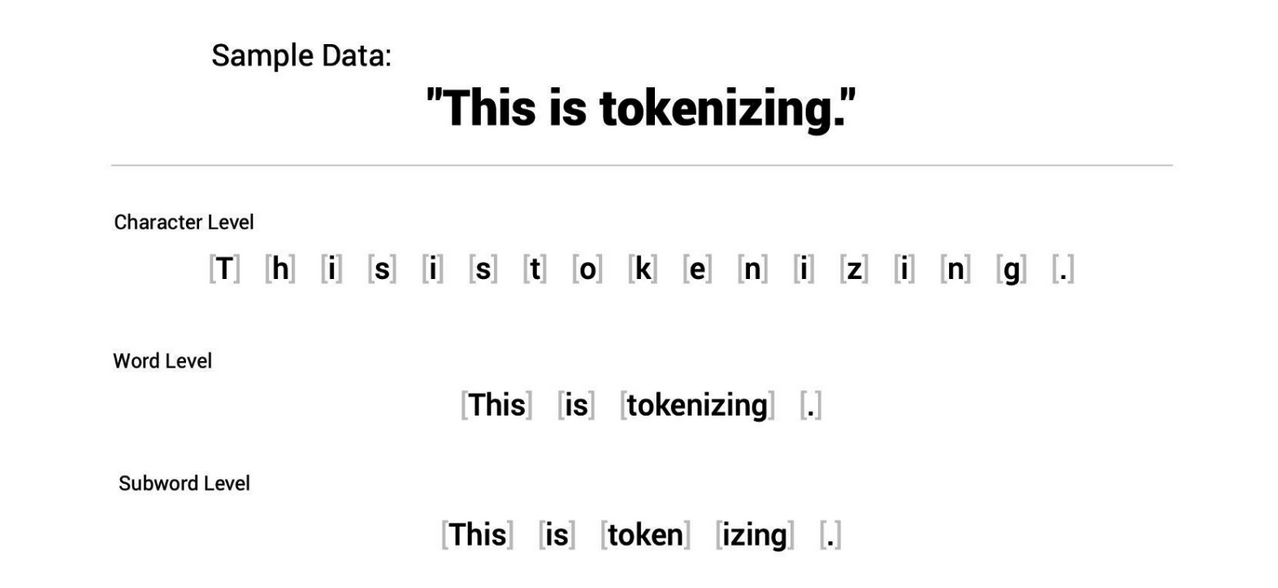
\includegraphics[width=0.5\textwidth]{Images/Tokenizer.png}
    \caption{Types of Tokens}
    \label{fig:example_image}
\end{figure}

While character and word level tokenization are obvious, subword level tokenization requires specific algorithms, such as Byte-pair encoding, WordPiece, and SentencePiece, to tokenize words. After the data is tokenized, the pre-training of the language model begins. Pre-training the step where researchers will train the model on the corpus of text completely unsupervised to help build its base ability to respond to inputs as well as assign probabilities to tokens. Now that the model is pre-trained and knows how to form general sentences, now the model is ready to be fine-tuned to perform specific tasks. To fine-tune a model is to then train it on a smaller, specific dataset that is more tailored to the task which the model is meant to solve. \\ \indent The key differences between Pre-Training and Fine Tuning are computational intensity, scale and scope of data, and the learning methods. In comparison to pre-training, fine tuning is significantly less intensive\cite{noauthor_25_nodate}. requires task specific labeled data sets, and its learning is supervised by humans. The reason for finetuning is because by original design large language models are not designed for user, so fine tuning allows language models to become more user friendly. \\ \indent Another part of training a large language model is Reinforced Learning by Human Feedback(RLHF)\cite{noauthor_what_2024}. Reinforced Learning by Human Feedback involves humans judging responses from a large language model based on a certain criteria. An example of this is people rating how funny a language model’s joke is. To incentivize a model to learn the patterns that humans have provided positive feedback on, a reward function is used to encourage models to reproduce target behaviors as well as create new responses that may try to trigger the function in new ways. Tokenization, pre-training, fine-tuning, and RLHF are all important steps in training a large language model.  

\subsection{Evaluation Metrics: Intrinsic and Extrinsic}
It is easy to see how well the language model itself runs in general. Whether it produces a well-formed sentence or so called “word salad” is a good indicator that a large language model is working correctly. However what is significantly harder to determine is how well one language model performs compared to another. In this vein there are two types of evaluations that can be done to compare the performance of two language models.\\ \indent The first type of evaluation is called intrinsic evaluation. Intrinsic evaluation captures how well a model captures what it is “supposed” to capture. Essentially the output of the language model is evaluated against its source material and measured for how closely it conveys that same message. To measure an intrinsic evaluation, scientists have used perplexity. Perplexity is defined as the inverse of the probability of a large language model’s test set then normalized by the number of tokens, or words, in the test set. What perplexity measures is how well a model reacts to the introduction of new, unseen data. The lower a model's perplexity is, the better the model reacts\cite{gandhi_evaluation_2020}. Here is a visual representation of the formula:
\\
\begin{figure}[h]
    \centering
    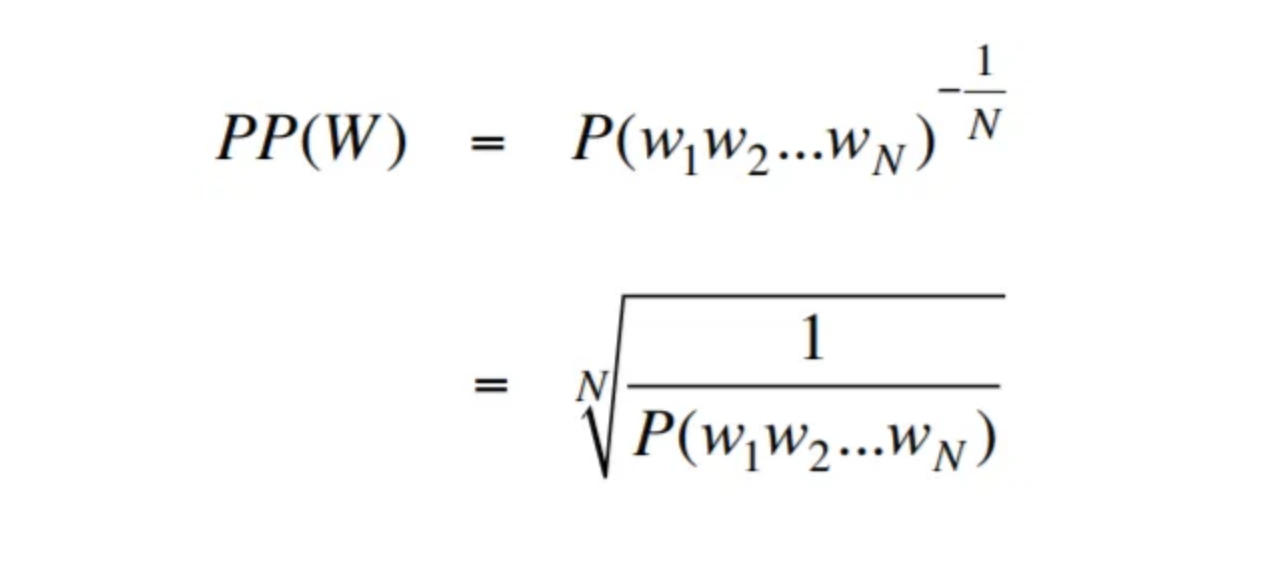
\includegraphics[width=0.5\textwidth]{Images/Perplexity.png}
    \caption{Perplexity Formula}
    \label{fig:example_image}
\end{figure}

The problem with this formula is because of how vast the test sets of language models can be, the probabilities of each word can be extremely small, so multiplying them all together can lead to arithmetic underflow. To combat this issue, the formula was re-written in logarithmic form, as seen below\cite{gandhi_evaluation_2020}: 
\\
\begin{figure}[h]
    \centering
    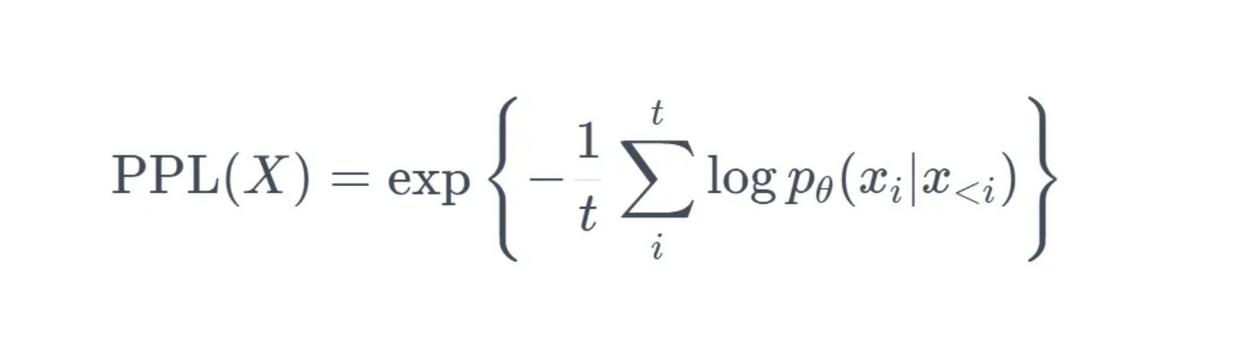
\includegraphics[width=0.5\textwidth]{Images/Log_Plex.png}
    \caption{Perplexity Formula: Logarithmic}
    \label{fig:example_image}
\end{figure}

There are other shortcomings of perplexity, but I will cover these issues in the potential concerns section of this paper. While perplexity can tell us how well a model takes in new information and how the language model assigns probabilities to the new information, it fails to communicate how well the language performs its actual task of conveying relevant and useful information to the user. To measure this, scientists use extrinsic, or task-based, evaluation.\\ \indent Extrinsic evaluation consists of training two separate language models and then having both of the models perform the same task, where their scores are measured and compared to determine which one provides the best information. Word Error Rate(WER) is the formula used to determine how accurate a model's text is. Originating from speech recognition, word error rate is the sum of the substitutions, deletions, and insertions needed to make the text into the actual transcription divided by the number of words in the reference. An insertion is the need to add a given token to the predicted sentence to make it correct. A deletion is the removal of a token to correct the predicted sentence. A substitution is the swapping of a token to correct a predicted sentence. Below is the formula for word error rate as well as examples of insertion, deletion, and substitution:

\begin{figure}[h]
    \centering
    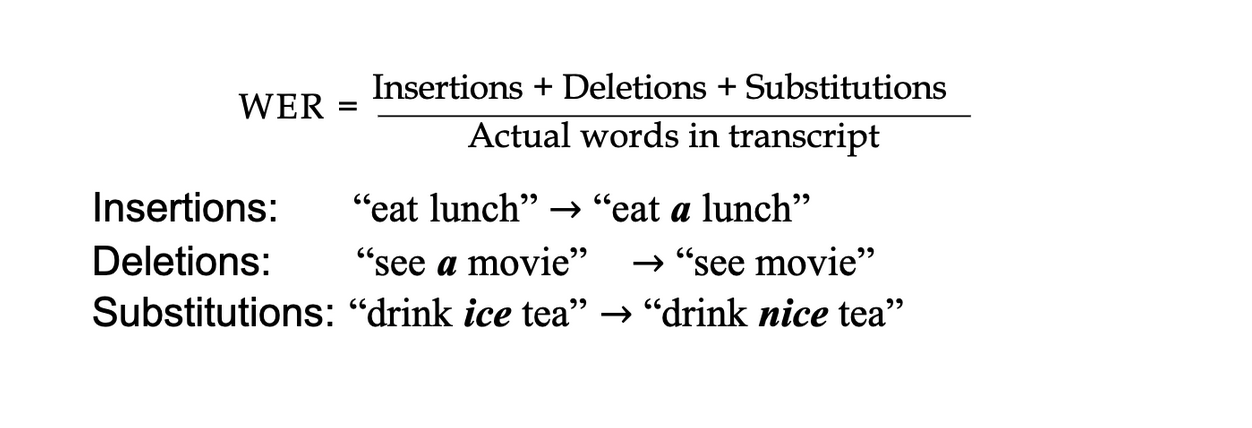
\includegraphics[width=0.5\textwidth]{Images/WER.png}
    \caption{Word Error Rate Formula}
    \label{fig:example_image}
\end{figure}

\subsection{Attention Mechanisms}
Later in this paper I will be discussing various types of Attention Mechanisms\cite{american_express_comprehensive_2019}. An Attention Mechanism works by comparing the similarity score, how related two data points are, of keys and queries. Below is a small example of what keys, queries and values are:\\ 


    
\indent Query: “What did John eat?”\\
\indent Potential Keys: “steak”, “apple”, “candy”, “sushi”\\
\indent The attention mechanism would go through each key  
\indent individually and rate them based on how similar they 
\indent are to the query, and the key with the highest score would 
\indent influence the final output.
\\



Now there is another method called “Multi-Head Attention” where multiple attention mechanisms are run parallel to one another, with “head” referring to an attention mechanism\cite{noauthor_papers_nodate}. To do this, the input is broken up and each head is given a part of the input to analyze. Running multiple heads parallel to each other allows the heads to create independent similarity scores that allow the model to capture unique relationships that a single head may not have been able to replicate. It is important to note that because this process is using multiple independent heads at the same time, this task can be both computationally and memory intensive.


\section{Prior Work}
Since the introduction of ChatGPT 3 in 2022, there has been an influx in new and fast large language models flooding the tech world. With so many different models to cover, I have chosen three specific models that I have done research into to discuss their contributions to the field as well as compare what I am attempting to do with what they have accomplished. The three models I will be talking about are ChatGPT, Google Gemini, and Mistral. 

\subsection{ChatGPT}
The first ChatGPT paper was written in June of 2018 titled “Improving Language Understanding by Generative Pre-Training”\cite{radford_improving_nodate}, about one year after the first official paper about transformers, the  backbone architecture of how ChatGPT and other current large language models work. The papers main points detail the relevance of using a transformer architecture, the pre-training and supervised fine tuning of the model as well as how data efficient the model was. While this paper is revolutionary, it is more about building the foundation of language models and less about their effectiveness. In February of 2019, OpenAI would publish the paper for GPT 2, titled “Language Models are Unsupervised MultiTask Learners”\cite{radford_language_nodate}. While most of the paper talks about improvements such as bigger parameters and improved scalability, the parts of the paper that piqued my interest most pertained to zero, one and few shot learning. Zero shot learning refers to how well a model performs a task with no instruction, purely using what it learns in pre-training.  An example of this would be to input a math equation like 2 + 2 with no context and see what the machine comes up with. On the other hand, one shot learning provides the model with one example of how to perform the task and then expects the machine to infer how to solve similar problems. This would be like telling the machine 1 + 1 = 2, and then inputting 2 + 2 and seeing what comes out. Lastly, few shot learning is the same as one shot learning but with multiple examples. The paper found that few shot learning had a profound effect on the performance. Upon further research into the subject, I found an article which claimed that when comparing few shot learning to fine-tuning, the few shot learning led to the model having an accuracy rating of 97 percent compared to the fine-tuning’s accuracy score of 91 percent\cite{noauthor_zero-shot_nodate}. However, the paper concluded that if there are few queries and that for larger-scale more repetitive tasks, it is worth fine tuning the model. This comparison of few shot learning and fine-tuning provided me with a new lens to look through when determining how I may choose to train my model. In May of 2020, OpenAI would release a paper about GPT 3, titled "Language Models are Few-Shot Learners". As the title of the paper suggests, the paper discusses how few shot learning has significantly improved overall performance of GPT, but also how GPT 3 itself has shown better performance in both zero and one shot learning. The paper also brings up two main concerns, the need for bias mitigation as well as the computational costs of fine tuning and training a language of its size. At this point, GPT 3 is around 175 billion parameters, whereas GPT 2 was 1.5 billion. While this has improved the performance of the model, it has led to the issue of bias in its responses as well as hallucinating incorrect facts. On top of these issues, the paper discusses how expensive it was to train a model of such size. It is estimated that the process of training GPT 3 cost more than 4 million dollars\cite{leswing_chatgpt_2023}. Finally, in March of 2023 OpenAI released a technical report for GPT 4. The article is much the same as the others, showing the performance of GPT 4 in various languages as well as mentioning that there is still bias and hallucination in its results. This report does not offer much that prior reports haven't covered. 

\subsection{Mistral}
First published in October of 2023, Mistral released their first paper “Mistral 7B”\cite{gathnex_mistral-7b_2023}. The paper claimed that despite having only seven billion parameters, this model was able to outperform others models with nearly twice or even five times the number of parameters in given categories, specifically citing Llama 2 and Llama 1 respectively. In the paper the authors detail how Mistral 7B takes advantage of two key ideas: Group Queried Attention\cite{noauthor_number_2023} and Sliding Window Attention\cite{noauthor_papers_nodate-1}. Group Queried Attention takes the idea of Multi-Head Attention but rather than having all heads run independently, it groups some of the heads together, reducing the number of individual computations needed thereby increasing the processing speed. Grouping the heads allows for an analysis near the level of Multi Head Attention without the extreme computational and memory inefficiencies. Similar to Group Queried Attention, Sliding Window Attention is another method to reduce inefficiencies while making the model scalable. In a traditional attention mechanism, every token from the input is allowed to interact with any other token to determine the output, a process which grows quadratically complex in respect to the string’s length. What Sliding Window Attention does is divide the input sequence into smaller “fixed windows” that overlap one another and allows tokens to interact with other tokens in their window. This significantly reduces computational complexity as well as ensures the smooth flow of information from the beginning to end of the sequence. With Group Queried Attention and Sliding Window Attention, Mistral 7B was able to outperform Llama 1 in all evaluation benchmarks with nearly half the number of parameters. When compared to Llama 2, which has 34 billion parameters, Mistral 7B was able to outperform it in reasoning, math, and code generation, despite being nearly a fifth the size.  

\subsection{Discussion}
In looking at the various papers on ChatGPT models one through four as well as the Mistral 7B paper, I have gained comprehensive insight into what makes an effective large language model as well as the issues one can face when making their own model. Their papers detail the importance of an unsupervised pre-training process to build a model’s general knowledge coupled with tailored fine-tuning to teach the model how to interact with input and react to input it is unfamiliar with via zero, one and few shot learning. These papers also taught me about architectural innovations like General Query Attention and Sliding Window Attention which allow for a smaller model to compete with the performance of models that are multiple times its size. In turn, I have learned about how as a language model grows the monetary and environmental costs of continuing to train it new information becomes exceedingly costly.

\section{Methods}
In this section, I will list my methods for how I intend to complete this project along with my reasons for why I chose one particular method over other methods listed prior in this paper or others that I will bring up when the time comes.

\subsection{Which Model to Use?}

While there are many language models to consider, with at least twenty five open large language models available at the moment, the main two models I chose to look at were ChatGPT and Mistral. While ChatGPT from version 3.0 onwards is undoubtedly more powerful than Mistral 7B, I have chosen to go forward and chose Mistral 7B to serve as the model I will train for my project. One of my main reasons for choosing Mistral over ChatGPT are its efficiency and accuracy despite its small number of parameters. This project will be run on my laptop as well as Occidental’s cluster. While the cluster is an incredibly powerful tool, its computational power is not solely dedicated to my project, but to projects done by various departments present at Occidental College. On top of its size, Mistral’s architecture, specifically Grouped Query Attention, makes it efficient even compared to other small language models and larger models too. Another reason why I like Mistral for my project is that it is entirely open source and accessible. This means I will be able to download my model and not rely on API calls like I would for GPT. This both gives me more control over the training and fine-tuning process as well as save money, as ChatGPT charges money for each API call made. Mistral is also better suited for my needs because it was designed to be fine-tuned for various tasks effortlessly \cite{gathnex_mistral-7b_2023}. Mistral 7B proves itself to be the best balance of efficiency and performance.


\subsection{Pre-Trained or Untrained?}

Because Mistral is an open source large language model, I have the option between choosing a model that has already been pre-trained or take an entirely empty model and pre-train it myself. The advantages of pre-training the model myself is having full control and understanding of what the model is being trained on so that I can better understand how it reaches its conclusions. While this would be ideal, there are two reasons why this is not very viable. The first reason is Occidental College does not have enough data. Between the three webpages and even the school newspaper, I do not believe there are seven billion parameters worth of information available for me to train a computer from scratch. On top of this, the purpose of pre-training is to create general knowledge, so it would be counterproductive to pre-train entirely on Occidental data. The last and most obvious reason is the sheer cost of pre-training a model. While I will have access to Occidental’s cluster to train the model, using it for pre-training could be extremely expensive as well as interfere with research in other departments. For these reasons, I have opted to use a pre-trained version of Mistral 7B and will instead attempt to analyze the data it was already trained on.

\subsection{Data Collection, Fine-Tuning, Tokenization, and User Testing}
As aforementioned, for my project I intend to collect data from Occidental’s main three websites: the Occidental Webpages, MyOxy, and Raftr. To do this I intend to use a python web scraper to collect all text and metadata from the websites and store them as plain text files. After collecting all of the data, I will use a subword tokenizer, as was used by ChatGPT, using a Byte-Pair Encoding on all of the data. Once tokenized, I will need to go through and start labelling the data in order to prepare it for fine-tuning. I expect that most of my time in summer will be spent doing this.  I intend to fine-tune the model on the tokenized data and use Reinforced Learning from Human Feedback to monitor and correct its output in order to teach it how to respond to questions from members of the Occidental community. I believe a considerable amount of my project's time will be spent on user testing and having people give feedback on how the model responds, and then adjusting the model accordingly. While I have no concrete method in mind, the current plan after fine-tuning will be to have members of the community ask the machine pre-scripted questions and rate its usefulness to them.


\section{Evaluation Metrics}

\subsection{Intrinsic Evaluation: }
To measure how coherent and accurate the model is to its source material, I will be utilizing the logarithmic version of the perplexity formula seen in the technical background section of this paper. I plan to have around ten set questions that I will ask during each evaluation and measure perplexity to see how well it accurately captures its source material. I will also evaluate how well the model handles some randomized prompts, which will be coherent sentences and see how it reacts to that. 

\subsection{Extrinsic Evaluation:}
On top of perplexity, I will also be evaluating each response from the model using the Word Error Rate formula from the technical background section. WER will be applied to the same ten prompts used for perplexity as well as the random prompts that I will throw in during each evaluation. Since WER is comparative by nature, I will compare the results to the base Mistral model as well as Llama1, Llama 2, and ChatGPT 3.0.


\section{Time Line}

\begin{itemize}
    \item \textbf{Summer 2024}
    \begin{itemize}
        \item Web scraping Occidental resources, labeling data, and tokenization
    \end{itemize}

    \item \textbf{August 2024}
    \begin{enumerate}
        \item Fine-tuning the data on the cluster*
        \item Fine-tuning the data on the cluster*
    \end{enumerate}

    \item \textbf{September 2024}
    \begin{enumerate}
        \item User testing and RLHF (Reinforcement Learning from Human Feedback)
        \item User testing and RLHF
    \end{enumerate}

    \item \textbf{October 2024}
    \begin{enumerate}
        \item User testing and RLHF
        \item User testing and RLHF
    \end{enumerate}

    \item \textbf{November 2024}
    \begin{enumerate}
        \item User testing and RLHF
        \item Creating a UI for users
    \end{enumerate}

    \item \textbf{December 2024}
    \begin{enumerate}
        \item Work on creating final version to show at the presentation
        \item Final touches / Submission
    \end{enumerate}
\end{itemize}

\noindent *Given that I do not know how many tokens I will end up with, it is hard to estimate how long fine tuning will take. The estimate I am working with is 6 hours for 5,500 tokens. To ensure I have time, I am giving myself an extra two weeks. If I finish earlier, I will start user testing ahead of schedule. \cite{noauthor_how_nodate}

\end{document}
